%Experimental Results and Analysis – in this section you should show the quantitative results – charts and tables. Analyze the results by explaining and highlighting what is important on them in terms of your goals and what is bad. You should explain the strange results too.

\section{Results and Analysis} 
\label{sec:results} 

TODO design a structure 

In this section we present and analyse our most important results. Other results could be seen in the appendix \ref{sec:appendix-results}. 

\subsection{Two learning rates} 
\label{sec:results-two-lambdas} 

For all models tested on the 4-2-4 encoder task~\ref{sec:datasets-auto4} the two lambda model~\ref{sec:our-two-lambdas} had the best success rate as shown on figure~\ref{fig:results-two-lambdas-auto4-success}. 

\begin{figure}[t]
  \centering
  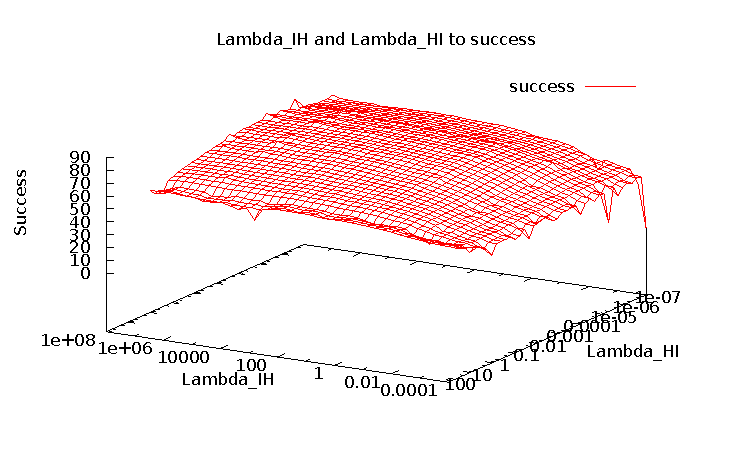
\includegraphics[width=0.8\textwidth]{img/success_to_lambdas.pdf}    
  \caption{Encoder 4-2-4: Performance of the two-lambda model with $\sigma = 2.3$ and $\mu = 0.0$.}
  \label{fig:results-two-lambdas-auto4-success}
\end{figure}
\begin{figure}[t]
  \centering
  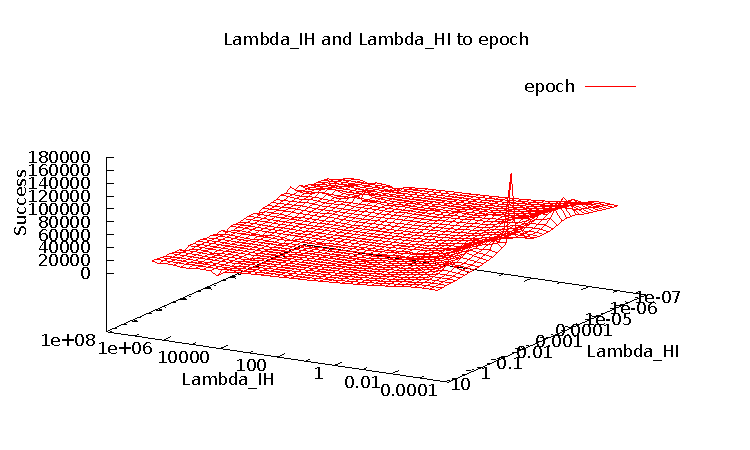
\includegraphics[width=0.8\textwidth]{img/epoch_to_lambdas.pdf}    
  \caption{Encoder 4-2-4: Convergence time of the two-lambda model with $\sigma = 2.3$ and $\mu = 0.0$.}
  \label{fig:results-two-lambdas-auto4-epoch}
\end{figure}

\subsection{Other} 
\begin{figure}[t]
  \centering
  \includegraphics[width=0.8\textwidth]{../bal/data/stats/test/epoch_to_err.pdf}    
  \caption{Encoder 4-2-4}
  \label{fig:TODO-1}
\end{figure}


\begin{figure}[t]
  \centering
  \includegraphics[width=0.8\textwidth]{../bal/data/stats/test/epoch_to_h_dist.pdf}    
  \caption{Encoder 4-2-4}
  \label{fig:TODO-2}
\end{figure}

% TODO forward backward error 
\begin{figure}[t]
  \centering
  \includegraphics[width=0.8\textwidth]{../bal/data/stats/test/epoch_to_success.pdf}    
  \caption{Encoder 4-2-4}
  \label{fig:TODO-3} 
\end{figure}

% TODO compare several models 
\begin{figure}[t]
  \centering
  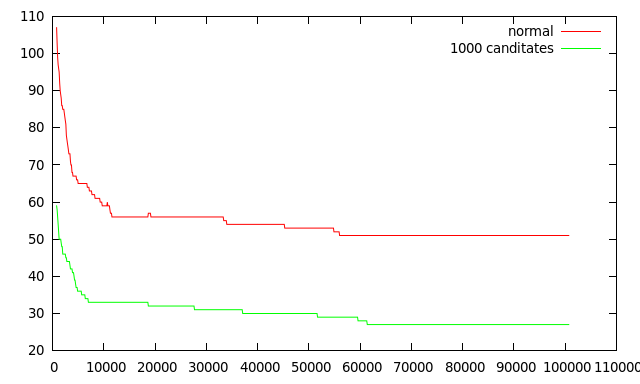
\includegraphics[width=0.8\textwidth]{../presentation/img/long_run_error.png}    
  \caption{Encoder 4-2-4 - Candidate selection vs. normal BAL}
  \label{fig:TODO-4}
\end{figure}

TODO hidden activation timelines (for each model) 

\subsection{Comparison} 

TODO: success / learning rate \\
TODO: epochs / learning rate  \\
TODO: success / epochs  \\
TODO: bitSucc and patSucc \\
TODO: success / hidden layer size  \\
 
\subsubsection{4-2-4 Encoder}
TODO as a plot {sec:datasets-auto4} 

\subsubsection{Complex Binary Vector Associations}
TODO as a plot {sec:datasets-k3} 
%09-12-2013
%\begin{itemize}  
%\item 3  - 79.5\%
%\item 4  - 94.9\%
%\item 5  - 98.5\%
%\item 6  - 99.5\%
%\item 7  - 99.8\%
%\item 8  - 99.9\%
%\item 9  - 100.0\%
%\item 10  - 100.0\%
%\end{itemize} 

\subsubsection{Hand--written digits.}
TODO simulation + plots \ref{sec:datasets-digits} 

%TODO Mathematical analysis of the last model - o'really clanok aproximacia gradientu chyby
\subsection{Analysis} 
\begin{itemize} 
\item Matrices IH-OH and HO-HI tend to be same in autoassociative tasks. 
\item Hidden representation distance is a meaningful measure (LinReg on pre\_measure) (+ 10\%) . 
\item In triangle (non-convex). Not-in triangle is a must to condition for success. \\
TODO rerun to get "1 err in\_triangle" with and without preselection (there was a bug in the old data). 

\item Long run (+ 10\%). It seems it's always better to have long runs.  
\item reprezentacie na hidden absolutne rovnake (forward, backward), matice rozne:
\item Convergence Epsilon - weights tend to infinity (09-12-2013: Convergence which depends on average weight change does not work). 
\item Rerun - same config, different order when training 
All bad: \\
err sigma lambda momentum success sample\_ratio \\
0.0 2.3 0.7 0.0 19.296918767507005 6889/35700 \\
1.0 2.3 0.7 0.0 68.05602240896359 24296/35700 \\
2.0 2.3 0.7 0.0 12.644257703081232 4514/35700 \\
3.0 2.3 0.7 0.0 0.0028011204481792717 1/35700 \\

All good:  \\
err sigma lambda momentum success sample\_ratio \\
0.0 2.3 0.7 0.0 99.98911353032659 64293/64300 \\
1.0 2.3 0.7 0.0 0.01088646967340591 7/64300 \\


\end{itemize}

\subsubsection{Convergence} 
TODO make it shorter 

24-02-2014
TODO: Measure in how many cases the learning ends with convergence (no weight change) and divergence (oscialtion of seveal states). 

 Mathematical background on convergence and learning rule: 

(Hopfield networks, Wikipedia) The requirement that weights be symmetric is typically used, as it will guarantee that the energy function decreases monotonically while following the activation rules, and the network may exhibit some periodic or chaotic behaviour if non-symmetric weights are used. However, Hopfield found that this chaotic behavior is confined to relatively small parts of the phase space, and does not impair the network's ability to act as a content-addressable associative memory system.

(O'Reilly 1996) The GeneRec Approximation to AP BP
The analysis presented earlier in the paper shows that GeneRec should compute the same error derivatives as the Almeida-Pineda version of error backpropagation in a recurrent network if the following conditions hold:
  The difference of the plus and minus phase activation terms in GeneRec, which are updated in separate iterative activation settling phases, can be used to compute a unit’s error term instead of the iterative update of the difference itself, which is what Almeida-Pineda uses.
  The reciprocal weights are symmetric. This enables the activation signals from the output to the hidden units (via the recurrent weights) to reflect the contribution that the hidden units made to the output error (via the forward-going weights).
  The difference of activations in the plus and minus phases is a reasonable approximation to the difference of net inputs times the derivative of the sigmoidal activation function. Note that this only affects the overall magnitude of the weight derivatives, not their direction.
  
(PINnc89.pdf) 

\paragraph{Generec-Bias} 
TODO: move to implementation? 

Therefore we tried several settings: 
\begin{itemize} 
\item No bias - two patterns for 4-2-4, three patterns for 4-3-4, all four patterns for 4-4-4
\item Bias only on the input layer:  
4-2-4 best network error = 3.0 (tended to have two very profiled (0.95+, 0, 0, 0) and two very even (0.5, 0.5, 0.5, 0.5)  \\
4-3-4 about 75\% success rate 
\item Bias on both input and hidden layers: 
    4-2-4 0.0 1.0 0.5 0.1 91.74311926605505 100/109, almost no 1.0 errors 
          epochs ranged from 9 to 4500 \\ 
    4-3-4 about 100\% succes rate with about 20 epochs (epoch ranged from 5 to 700) 
\item Bias on all matrices (IH, HO, OH): 
    seems to add a little chaos with a slighty worse performance (but maybe bad sigma)

\end{itemize} 

$$r_x\frac{dx_i}{dt} = -x_i + \sum_j w_{ij} f(x_j) + I_i$$
TODO: Frome where comes this equation? 

There are several ways to guarantee convergence. One way is to
impose structure on the connectivity of the network, such as requiring
the weight matrix to be lower triangular or symmetric. Symmetry, al-
though mathematically elegant, is quite stringent because it constrains
microscopic connectivity by requiring pairs of neurons to be symmetri-
cally connected. A less stringent constraint is to require that the Jacobian
matrix be diagonally dominant. For equation (2.11, the Jacobian matrix
has the form: 

$$L_{ij} = \delta_{ij} - w_{ij}f'(x_j)$$
Guez et al. (1988) 

(PINnc89.pdf) then the gradient descent dynamics will not change the stability of the network. The need
for this assumption can be eliminated by choosing a dynamical system
which admits only stable behavior, even under learning, as was done by
Barhen et al. (1989). TODO look up Barhen et al. (1989) article 

TODO - general theorem concerning staiblity of networks with symmetric weights Cohen and Grossberg 1983 

GLOBAL ASYMPTOTIC STABILITY - the network will settle for any input 
FIXED POINT =similar= MEMORY

(pineda1987) Oscilation (on recurrent BP) could occur when substantial SELF-EXCITATION 

\subsubsection{High-dimensional data} 
TODO!! analysis of high-dimensional data (CBVA, HandWritten) 
It's not most relevant if only 4-2-4 was analysed. 

\subsection{TODO} 

\subsubsection{Measure - Weight decay}
A commonly-used bias or regularizing function is weight decay (e.g., Hinton, 1989a; Weigend et al., 1991).
We implemented two commonly-used forms of weight decay in the Bp and GeneRec networks, simple
weight decay and weight-elimination weight decay (Weigend et al., 1991). In simple weight decay, a con-
stant fraction of the weight value is subtracted at each weight update, and weight-elimination is similar
except that the rate of decay is a more complex function of the weight such that larger weights suffer rela-
tively less decay than smaller ones (supporting a prior assumption of a bimodal distribution of weight values
— one population of larger weights that are actually useful and another of near-zero weights that are not
useful; see Weigend et al., 1991 for details).
The results with these forms of weight decay for the 100 hidden unit network are shown in Figure 5.
Although a small amount (.002; smaller amounts had progressively smaller effects) of simple weight de-
cay appears to reliably improve generalization performance in both Bp and GeneRec, the difference is not
substantial. The weight-elimination version of weight decay always appears to impair, rather than improve,
performance. Although the specific forms of weight decay explored here were not overly successful in
this task, it is possible that other forms might perform better. Nevertheless, most forms of weight decay
\citet{o2001generalization} 

\subsubsection{Measure - Weight patterns} 
An examination of the weights in the trained networks clearly shows why generalization is impaired in the
interactive network (Figure 6). The units have not carved the input/output mapping into separable subsets
that can be independently combined for the novel testing items — instead, each unit participates in the
input/output mapping for multiple slots. Although this is true for both the backpropagation and GeneRec
networks, it is particularly damaging for the interactive GeneRec network because of its attractor dynamics.
In contrast, the feedforward backpropagation network is still capable of producing a roughly linear combi-
nation of hidden unit activations that yields reasonable (though far from perfect) levels of generalization. \citet{o2001generalization} 

Figure 7: Average pairwise overlap (normalized dot product or cosine) between hidden patterns corresponding to
inputs that differ by a) 75\% (1 out of 4 slots different) and b) 50\% (2 out of 4 slots different). Feedforward back-
propagation (Bp) remains much closer to a linear response level (75\% and 50\% hidden similarity, respectively) after
training compared to interactive GeneRec, which shows evidence of attractor dynamics pulling the network away from
a linear, combinatorial response to the inputs.

\subsubsection{Mathematics} 
\begin{itemize} 
\item dynamic systems 
\end{itemize}

